\documentclass[a4paper,10pt]{article}
\usepackage[margin=2.7cm]{geometry}

% load package with some of the available options - you may not need this!
%\usepackage[framed,numbered,autolinebreaks,useliterate]{mcode}
\usepackage[framed,numbered,autolinebreaks]{mcode}
\renewcommand{\lstlistingname}{Code}
\newcommand{\figdir}{../../../fig/sigInspect}
\usepackage{graphicx}

% no section numbering
\setcounter{secnumdepth}{0}
% set TOC levels
\setcounter{tocdepth}{2}



% something NOT relevant to the usage of the package.
\usepackage{url,textcomp}
\setlength{\parindent}{0pt}
%\setlength{\parskip}{6pt}

\renewcommand{\arraystretch}{1.2} % increase table cell spacing




\title{sigInspect User's Manual}
\author{Eduard Bakstein, \emph{eda@zzz.cz}}
% //////////////////////////////////////////////////

\begin{document}

\maketitle

\begin{center}
\begin{minipage}{.75\linewidth}
%	\textbf{INSPECTION OF MICROELECTRODE RECORDINGS MADE SIMPLE}

\verb|sigInspect| is a Matlab GUI tool for inspecting multi-channel recordings. Is particularly useful for extracellular microelectrode recordings and allows \emph{visualization}, \emph{playback} and \emph{annotation} of segments containing \emph{artifacts}.

SigInspect was developed by the NEURO group (\url{http://neuro.felk.cvut.cz}) at the Department of Cybernetics, Faculty of Electrical Engineering, Czech Technical University in Prague.
	
\end{minipage}
\end{center}

\tableofcontents
\vspace{1.5em}
\section{Overview}
\verb|sigInspect| is a graphical user interface (GUI) application for Matlab, developed for inspection and annotation of extracellular microelectrode recordings (MER). The tool allows concurrent visualization of multiple parallel channels, playback and spectrogram plot of selected channels (to identify specific firing patterns) and especially annotation of individual channels. Parallel signals are displayed in one-second segments, which can be easily annotated using the GUI controls or shortcut keys.

SigInspect also contains tools for \textbf{automatic annotation of microelectrode recording data}, based on published methods. This can provide starting point for manual annotation and speed up the data-cleaning process considerably.

\newpage

\section{Quick start}

\subsection{Signal}
A signal in \verb|sigInspect| is assumed to be a \textbf{row vector} with samples in columns, a \textbf{multi-channel signal is a matrix with channels in rows}. SigInspect shows always one second segment of all channels in current signal. A signal can have one to unlimited number of channels.

\subsection{Loading a signal - the simple way}
The simplest way to start viewing and annotation is to call \verb|sigInspect| with signals as a parameter. Multiple signals can be passed in a cell array instead - user can then choose the displayed signal using the "signal" selector. The second parameter is sampling frequency in Hz (default value: $24 kHz$ is set if second parameter is omitted)
%[caption=Simple ways to load a signal, label=codeSimpleLoad]
\begin{lstlisting} 
% 1 - single multi-channel signal (matrix as input)
size(signal)					   % C x N matrix (C = channels, N = samples )
sigInspect(signal, samplingFreq);  % signal: chan. in rows, samples in columns

% 2 - multiple signals (cell array as input) 
s={signal1,signal2,signal3}; 
sigInspect(s, samplingFreq); 
\end{lstlisting}

\subsection{Loading signals from a mat-file}
In case \verb|sigInspect| is called without parameters, an \emph{Open file dialog} will pop up upon intialization, asking you to select a \mcode{*.mat} file with data. The mat-file has to contain signals in a cell array - the format described above - in \textbf{a variable called signal, signals or data}. Otherwise, your signals will not be found and the application will issue an error.

\begin{figure} [htb]
\centering
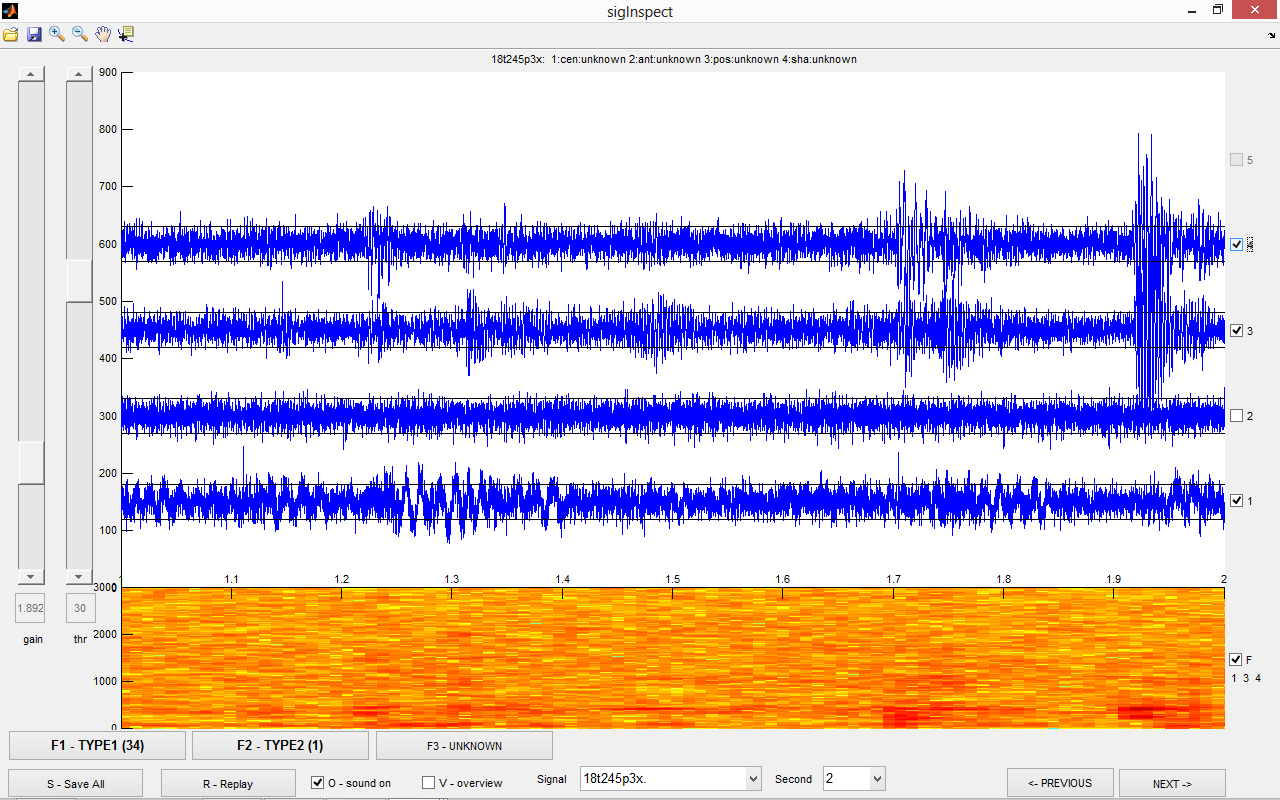
\includegraphics[width=1\textwidth]{sigInspectExploratory.png} 
\caption{Main window of the sigInspect GUI with loaded 4-channel signal}
\label{fig:sigInspectMainWindow}
\end{figure}

\subsection{Using the GUI}

The sigInspect GUI with loaded signals can be seen in Figure \ref{fig:sigInspectMainWindow}. The main window consists of \emph{time series plot} with selected second of given (multi-channel) signal and \emph{spectrogram}, calculated from currently selected channels.


\subsubsection{Basic controls}
\textbf{Switching between seconds} can be done using the $\leftarrow$ left and right $\rightarrow$ arrow keys. When you reach the last second of current signal and hit right, you get to the first second of subsequent signal and vice versa. You can of course use corresponding buttons called "previous" and "next" or "signal" and "second" selector boxes with the same effect.

To have a clear view of all your channels, you will probably need to \textbf{adjust gain} (amplitude) of the signals. This can be done either by the "gain" slider on the left or by pressing $\uparrow$ up or $\downarrow$ down arrow keys.

\subsubsection{Channel selection}
There are several operations that affect only the selected channels A) annotation (when you mark a specific 1s signal segment as an artifact) B) audio playback (when audio is on) and C) spectrogram calculation. \textbf{Channel selection} can be done using the numpad keys (1-9), number keys (top row of your keyboard with ENG layout)\footnote{Number shortcuts work obviously only up to 10 channels (tenth channel is controlled by 0)} or with checkboxes on the right, next to each signal. You can also \textbf{invert selection} using the "i" key or \textbf{select all} with the "a" key.

\subsubsection{Audio}
SigInspect allows \textbf{playback of thresholded signals}, which is useful for artifact identification, as well as for simple overview of neuronal activity\footnote{This method is commonly used in Deep Brain Stimulation surgery for nuclei identification}. To hear audio playback, "Sound on" checkbox at the bottom has to be checked (use "o" shortcut to toggle sound), at least one channel must be selected and threshold has to be set lower than at least some parts of some of the selected channels. \textbf{Threshold} is indicated by the black horizontal lines surrounding each channel in the time series plot and can be adjusted by the "thr" slider on the left or by hitting the  $+$ and $-$ keys. SigInspect \textbf{plays only signal parts exceeding currently set threshold in selected channels}. This can be used to play back only firing patterns of close neurons. If you wish to hear the whole signal including neuronal background, set threshold to 0;

If you wish to \textbf{replay} current second, use the "r" key, hit "Replay" button or change channel selection.

\subsubsection{Annotation}
Annotation can be done by the artifact type buttons at the bottom or corresponding "F1"-"F12" keys. The number and types of artifacts are up to you and correspond to the ARTIFACT\_TYPES field in the settings. \textbf{When you hit a button, you assign it to all currently selected channels}. If the currently selected channels have this artifact type already assigned, you will unmark them. \textbf{You can assign from zero to all your defined artifact types to each second of each channel}. The labels on each button also show numbers of all selected channels, that have given artifact assigned.

Annotation can be \textbf{saved to a \mcode{*.mat} file} either by clicking the save icon in the toolbar, the "Save all button at the bottom" or by hitting "s". By default, annotation is saved to current directory as \mcode{ sigInspectAnnotyyyy-mm-dd-HHMMSS.mat}, where yyyy-mm-dd-HHMMSS is current date and time (to change this, see ANNOT\_DEFAULT\_FILENAME in the settings). Annotation can be loaded from a mat-file using the load icon in the toolbar.

The \textbf{format of saved annotation} is a cell array of the same length as the number of signals. Each cell contains annotation for given multichannel signal in a $C \times S\times A$ logical matrix, where $C$ is the number of channels, $S$ signal length in seconds and $A$ number of defined artifact types. For example, \mcode{annotation(3,2,1);} is one when the 3rd channel contains artifact of type 1 in 2nd second. Saved annotation also contains interface type, artifact types and signalIds to verify that you are loading annotation that fits to currently loaded data (when metadata do not fit, sigInspect offers you to match/repair the metadata).

If you switch the overview window on, you can also show signal segments annotated as artifact in color.

\subsubsection{Overview window}
By checking the "overview checkbox" or by typing "v" you turn on the overview window, which \textbf{shows whole current multi-channel signal}. Current second is marked by red rectangle - you can select any second by clicking on it in the overview window.

\begin{figure} [htb]
\centering
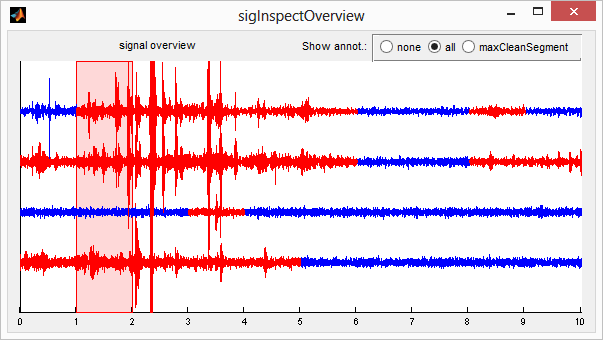
\includegraphics[width=.6\textwidth]{sigInspectOverview.png} 
\caption{Overview window showing 4-channel signal from Figure \ref{fig:sigInspectMainWindow} with  annotation}
\label{fig:sigInspectOverviewWindow}
\end{figure}

The overview window \textbf{can also display annotated artifacts} - just select the "all" radio button at the top. All clean segments with no artifact assigned will remain in default color (blue), while artifact seconds will turn red (can be changed in the settings). 

To see how long is the current \textbf{longest artifact-free segment}, select maxCleanSegment radio button. This will mark all shorter clean segment red, so that you have a quick idea how long clean contiguous segment of your signal is left.

The overview window uses further resampling to speed up display (see OVERVIEW\_DECIMATE\_FACTOR in the Settings section of this guide)

\subsubsection{Keyboard shortcuts}
For the sake of speed and usability, many controls can be accessed through simple keyboard shortcuts (mostly single-button). Most of the shortcuts are written directly in the GUI: you can e.g. press "o" to toggle sound on/off, "f" to toggle spectrogram or hit number keys to select or deselect channels.

\subsection{Settings}
To accomodate sigInspect to your needs, it may be necessary to alter some of its default settings. If you use your own data interface , the settings can be changed easily from there (see the "Advanced data loading" Section for more details). If you use sigInspect without defining your own \mcode{sigInspectDataInterface}, you can change settings easily using example code in Section \emph{Default interface}. 

All the main available settings are summarised in Table \ref{tab:sigInspectSettings} - the most important ones are in bold.

%%%%%%%%%%%%%%%%%%%%%% SETTINGS TABLE %%%%%%%%%%%%%%%%%

\begin{table}
\caption{Overview of available sigInspect settings}
\label{tab:sigInspectSettings}
\small
\begin{tabular}{p{.3\textwidth}cp{.4\textwidth}}
field name & default value & meaning\\
\hline
\multicolumn{3}{l}{basics \& signal handling} \\
\hline
\textbf{SAMPLING\_FREQ} & \mcode{24000} & signal sampling frequency in Hz \footnote{Note that when you are initializing sigInspect with a cell array of signals or with a path to a matfile, you can pass sampling frequency in Hz as the second parameter}\\
\textbf{PLOT\_STEP} & \mcode{ 150}                & distance on the y axis between channels \\
\textbf{PLOT\_CHANNELS} & \mcode{ 5 }             & max. number of prallel channels to plot  \\


DECIMATE\_FACTOR & 1 & decimate signals by this factor upon load (e.g. to save memory \& processing time)\\
ADAPT\_GAIN\_TO\_SIGNAL & 1 & automatically adapt gain slider to signal \\
ADAPT\_GAIN\_QUANTILE &  \mcode{.002}     & use this quantile of signal amplitude for gain adaptation \\

NORMALIZE\_SIGNAL\_PER\_CHANNEL  & \mcode{1} & normalize each channel (parallel signal) separately  \\
NORMALIZE\_SIGNAL\_PER\_CHANNEL \_QUANTILE & \mcode{0.1};       & use this quantile of signal amplitudes for per-channel normalization \\
\textbf{ARTIFACT\_TYPES} & $\lbrace$ \mcode{'ARTIF','UNSURE'}$\rbrace$ &  cell array with artifact type abbreviations (max TODO types) \\
ARTIFACT\_COLOR & \mcode{'r'}            &  color to plot artifact segments (shown in overview only) \\
ANNOT\_DEFAULT\_FILENAME & \mcode{'sigInspectAnnot##.mat'} & default name for sigInspect annotation when save button is hit. \#\# is replaced by current date and time \\

% time series plot
SHOW\_SIG\_INFO & \mcode{ 1}              & show signal  info from interface\\

\hline
\multicolumn{3}{l}{overview window} \\
\hline

OVERVIEW\_DECIMATE\_FACTOR & \mcode{ 20}  & decimate signals by this factor before view in the overview window - this is multiplied with the basic DECIMATE\_FACTOR \\
OVERVIEW\_GAIN & \mcode{ 10}             & increase gain in overview window (to adapt for decimation) \\

\hline
\multicolumn{3}{l}{spectrogram plot} \\
\hline

% spectrogram
SPECTROGRAM\_NFFT & \mcode{ 1024 }       & points to be used in spectrogram FFT. Window length is set to the same value, overlap is 50\% \\
SPECTROGRAM\_FREQ\_LIMS& \mcode{[0 3000]} & limit spectrogram to this frequency range - in Hz \\
DISABLE\_SPECTROGRAM & \mcode{ 0}        & disable spectrogram (will use the free space for signal plot) \\

ENABLE\_WHOLE\_SPECTROGRAM & \mcode{[0]} & Adds a 'w' toggle to switch between current second and whole signal spectrogram (Beta) \\



\hline
\multicolumn{3}{l}{audio} \\
\hline

% audio
START\_WITH\_SOUND\_ON & \mcode{ 0}        & start with sound turned on \\
USE\_BEEP & \mcode{0}             & beep when going to another signal \\
USE\_AUDIOPLAYER & \mcode{1}           & use audio playback by audioplayer (matlab audioplayer instead of play()) \\
PLAY\_VIA\_INTERNAL\_PLAYER & \mcode{1}          & use more sophisticated audio - may prevent audio dropouts and other problems on some systems \\
INTERNAL\_PLAYER\_DBG& \mcode{0}                 & show debug messages from internal player (works only if audioplayer is chosen \\
PLAY\_SOUND\_IN\_SYNC & \mcode{ 0}      & synchronized audio mode \\
CHECK\_CONST\_SAMPLES& \mcode{1}          & check signal for constant samples - visualize them in color \\

\hline
\end{tabular}
\end{table}

%%%%%%%%%%%%%%%%%%%%%% END SETTINGS TABLE %%%%%%%%%%%%%%%%%



\section{Advanced data loading - sigInspectDataInterface}
To provide the possibility to connect sigInspect to your existing database and to make configuration for multiple data sources easy, you can implement the \mcode{sigInspectDataInterface} and connect the GUI to whatever data source you are using. When you call sigInspect, you simply provide an instance of your implemented interface as the only parameter.

The two main things you have to implement are two methods: \mcode{getSignalIds()} which returns a list of signal identifiers (a cell array of strings) and \mcode{getSignalsById(signalId)}, which returns a (multi)channel signal matrix for given signalId. You can also override the default settings within your interface - this way, you can easily adapt sigInspect for multiple data sources you work with. Even though the Object programming is not very common in Matlab, implementing your own interface is very simple, as you will see below.

\subsection{In OOP terms}
In Object Oriented Programming (OOP) terms, such as in Java, the \mcode{sigInspectDataInterface} is an interface\footnote{in Matlab it is in fact an \emph{abstract class} as the language defines no interfaces and ignores the subtle distinctions between the two} you have to inherit in your own class. This is done in Matlab using the "$\langle$" sign after your function name. The \mcode{sigInspectDataInterface} has two abstract methods \mcode{getSignalIds()} and \mcode{getSignalsById(signalId)} which you have to implement to have a valid class. It may be also useful to define a constructor for your class, which allows you to e.g. pick data to view right on the object initialization. You can see an example class below.

\subsection{Reference}
\subsubsection{getSignalIds}
\begin{lstlisting}
function signalIds = getSignalIds(obj)
\end{lstlisting}
\mcode{signalIds} is a cell array of strings - unique signal identifiers. This function is called only once during sigInspect initialization. After that, sigInspect stores the signalIds internally.

\subsubsection{getSignalsById}
\begin{lstlisting}
function [signals chInfo]= getSignalsById(obj,signalId)
\end{lstlisting}
This function is called whenever the viewed signal changes and new one has to be loaded. Here, \mcode{signals} is a $C \times N$ matrix, where $C$ is the number of channels and $N$ is the number of samples. Thus, all channels have to be of the same length - use trailing zeros if one of the channels is shorter. The other output \mcode{chInfo} is a single string, which is shown in time series plot title. You can use this parameter to provide info about individual channels (such as in Figure \ref{fig:sigInspectMainWindow}, all text beyond the '18t245p3x:' (signalId) in the plot title.). If you do not need additional signal info, just return empty string.

\subsubsection{settings}
The last attribute of the abstract class is the \mcode{settings} structure. By default, this is an empty structure (i.e. it is not abstract), so you do not have to define within your interface. However, it may be very useful for defining settings for your data source. Settings are defined simply by assigning the settings structure a field of the same name as the property you want to change. For example, you can change the sampling frequency within your interface as follows:

\begin{lstlisting}
intf=myInterface();
intf.SAMPLING_FREQ=10000;
sigInspect(intf);
\end{lstlisting}

\newpage
\subsection{Example interface}
The following example code creates an interface to load signals from all csv files, present in a directory. In this example, the csv files contain three-channel micro-EEG signal in columns. The example ignores error checking (dir/file existence) for the sake of brevity.
\begin{lstlisting}
classdef sigInspectDataCsv < sigInspectDataInterface 
    % define class, inherit sigInspectDataInterface abstract class
    properties
        dirPath='';
    end
    methods
        % constructor - just store the path, set settings
        function obj=sigInspectDataCsv(dirPath)
            obj.dirPath = dirPath;
            obj.settings.SAMPLING_FREQ=6000; % 6kHz sampling rate
            obj.settings.PLOT_STEP=1.5;      % distance between channels on the y-axis
            obj.settings.ARTIFACT_TYPES={'Type A','Type B','Unsure'};            
        end        
        % return list of signal ids - load all csv files from a directory,
        % use filenames as signalIds
        function signalIds = getSignalIds(obj)
            lst=dir([obj.dirPath '/*.csv']);
            signalIds = {lst(:).name}';
        end
        
        % read signals based on signalId (=filename)
        function [signals chInfo]= getSignalsById(obj,signalId)
            chInfo='';
            signals=csvread([obj.dirPath '/' signalId]);
        end
    end
end
\end{lstlisting}
\subsubsection{Using the interface}
Once you have your class implemented, it is very easy to use it
\begin{lstlisting}
% initialize interface using its constructor
intf=sigInspectDataCsv('csvDemo/'); 
% change additional settings (optional)
intf.settings.NORMALIZE_SIGNAL_PER_CHANNEL = 0;
% run sigInspect
sigInspect(intf)
\end{lstlisting}

\subsection{Default interface: sigInspectDataBasic}
When you provide sigInspect with a cell array of signals or a path to a mat-file with data, it will initialize the default interface: \mcode{sigInspectDataBasic}, which accepts these on the input (see inline help for details). The main disadvantage of calling sigInspect with signals directly is that you have no possibility to change settings, other than to hard-code them in \mcode{sigInspect.m} directly. A simple workaround is to initialize the basic interface yourself as follows:
\begin{lstlisting}
% prepare data + initialize the Basic interface
signals = {signal1 signal2 signal3};
intf = sigInspectDataBasic(signals);
% change the settings
intf.settings.ARTIFACT_TYPES={'Wavy','Spiky','Other'};
% run sigInspect
sigInspect(intf);
\end{lstlisting}


\section{Automatic artifact annotation (Beta)}
To assist you with manual artifact annotation in your signals, the sigInspect tool provides you with several methods of artifact detection. This tool is fine-tuned for microEEG data and in its initial release, it is intended as a starting-point for manual signal inspection, rather than as a stand-alone tool. The workflow is following:
\begin{enumerate}
 \item initialize data interface of your choice 
 \item run \mcode{sigInspectAutoLabel} on this interface, which will result in automatic annotation in a mat-file.
 \item run \mcode{sigInspect} with the same interface, load the annotation
 \item update the artifact annotation manually to your taste
\end{enumerate}

To see different argument types of \mcode{sigInspectAutoLabel}, check out its inline help. For example, your artifact labelling code could look like this:

\begin{lstlisting}
% use the Basic interface + data in mat-file
intf = sigInspectDataBasic('mySignals.mat');
% change the settings
intf.settings.ARTIFACT_TYPES={'Automatic','MyArtif1','MyArtif2'};
% run autoLabel with the default method
sigInspectAutoLabel(intf,'myAutoAnnot.mat');
% run sigInspect
sigInspect(intf);
% now click the "load" icon in the toolbar and open myAutoAnnot.mat
\end{lstlisting}

\subsection{Artifact types handling}
No matter what artifact types you set in your interface, the  \mcode{sigInspectAutoLabel} function uses only 0-1 (clean-artifact) classification. The number of artifact types you define will only be used to resize annotation matrix for each signal to appropriate dimension. It may be a good idea to use artifact types in the form \mcode{intf.ARTIFACT_TYPES=\{'AUTO','myType1','myType2'\}}, so that you keep record of the original automatic annotation.

\subsection{Artifact classification methods}
While \mcode{sigInspectAutoLabel} is gateway function for user's convenience, artifact classification itself is performed by the function  \mcode{sigInspectClassify}. This function also implements all classification methods mentioned below. Artifact classification is done on a set of features computed from the raw signal by \mcode{sigInspectComputeFeatures} - the feature set varies from method to method.

\subsubsection{psd - deviation from ideal spectrum}
The \emph{psd} method is designed to detect artifacts with very strong frequency components and is based on our 2015 EMBC paper \cite{Bakstein2015}. The classifier stores a mean Power spectrum (or Power Spectral Density - PSD), calculated on clean portions of a training set of 60 ten seconds long microEEG recordings. Manual annotation of the training data was performed by 5 trained experts using previous version of the sigInspect tool. Classification threshold was set to maximum accuracy on the training data. More details can be found in the paper.

\subsubsection{Other methods}
Other more accurate classification methods are still under development. Please, stay tuned.
%\subsubsection{tree - decision tree classifier}
%This method uses a decision tree classifier

\section{About + license}
SigInspect is distributed under the Lesser General Public License (\url{https://www.gnu.org/licenses/lgpl-3.0.en.html}), which means you can use sigInspect free of charge for research, educational, commercial or any other purpose, but you should keep the license when using larger portions of the code. If you publish results processed with our tool, we expect you to give us appropriate authorship credit (e.g. by citing our paper \cite{Bakstein2015}). 

We will be very happy if sigInspect helps you in your research. If you are happy (or unhappy) with our tool, we will be glad if you let us know!


\section{FAQ}
\begin{description}
	\item[What does sigInspect do?] sigInspect is a Matlab GUI tool that Allows you to inspect and annotate multi-channel signals.
	\item[Can I start sigInspect without signals?] No, signals or interface must be provided on startup
	\item[Can I change interface during runtime?] No, this is currently not supported
	\item[Signals are overlapping, what shall I do?] You can A) change signal gain using +/- keys or slider on the left or B) change the PLOT\_STEP settings field
\item[What is the \emph{interface}?] The term \emph{interface} refers here to an object of class \mcode{sigInspectDataInterface}, which can be used to tailor the GUI to multiple data sources - see the "Advanced data loading" section for details.
\item[Do I need the \emph{interface}?] No, you do not have to worry - just start the sigInspect the basic way (with signals as a parameter), it will initialize \mcode{sigInspectDataBasic} interface for you.

	\item[Can I annotate segments shorter than the whole current view (1s)?] No, this is not possible. But trust us - this way it is \textbf{much} faster and it may also be really hard to identify beginning and end of an artifact.
\end{description}

\begin{thebibliography}{9}	
\bibitem{Bakstein2015}
	Bakstein E., Schneider J., Sieger T., Novak D., Wild J. and Jech R.
	\emph{Supervised Segmentation of Microelectrode Recording Artifacts Using Power Spectral Density}
	Proceedings of the 37th Annual International Conference of the IEEE Engineering in Medicine and Biology Society
	Milan, Italy,
	August 2015
	
\bibitem{Falkenberg2003} J. H. Falkenberg and J. McNames, \emph{Segmentation of extracellular microelectrode recordings with equal power} in Proceedings of the 25th Annual International Conference of the IEEE Engineering in Medicine and Biology Society, 2003, vol. 3, pp. 2475–2478.

\bibitem{Aboy2006} M. Aboy and J. H. Falkenberg, \emph{An automatic algorithm for stationary segmentation of extracellular microelectrode recordings} Med. Biol. Eng. Comput., vol. 44, no. 6, pp. 511–515, Jun. 2006.
	
\end{thebibliography}


\end{document}